% !TeX root = ./main.tex
\documentclass[letterpaper]{article}

\usepackage[spanish,es-tabla]{babel}
\usepackage[table,xcdraw]{xcolor}
\usepackage[nottoc]{tocbibind}
\usepackage{graphicx}
\usepackage{hyperref}
\usepackage{subfiles}
\usepackage{fancyhdr}
\usepackage{float}
\usepackage[left=3cm,right=3cm,top=3cm,bottom=4cm]{geometry}
\usepackage[acronym, toc, style=indexgroup]{glossaries}
\usepackage{hyperref}
\usepackage{multicol}
\usepackage{pdfpages}



\pagestyle{fancy}
\fancyfoot[R]{\thepage}
\fancyfoot[C]{
\includegraphics[width=0.1\textwidth]{inge_logo}}
\fancyhead[L]{\leftmark}
\fancyhead[R]{\rightmark}


\graphicspath{
  {img/}{images/}
}

\makeglossary{}
\documentclass[letterpaper]{article}

\usepackage[spanish,es-tabla]{babel}
\usepackage[table,xcdraw]{xcolor}
\usepackage[nottoc]{tocbibind}
\usepackage{graphicx}
\usepackage{hyperref}
\usepackage{subfiles}
\usepackage{fancyhdr}
\usepackage{float}
\usepackage[left=3cm,right=3cm,top=3cm,bottom=4cm]{geometry}
\usepackage[acronym, toc, style=indexgroup]{glossaries}
\usepackage{hyperref}
\usepackage{multicol}


\pagestyle{fancy}
\fancyhead[L]{\thepage}
\fancyfoot[C]{
\includegraphics[width=0.1\textwidth]{inge_logo}}



\graphicspath{
  {img/}{images/}
}

\makeglossary{}
\documentclass[letterpaper]{article}

\usepackage[spanish,es-tabla]{babel}
\usepackage[table,xcdraw]{xcolor}
\usepackage[nottoc]{tocbibind}
\usepackage{graphicx}
\usepackage{hyperref}
\usepackage{subfiles}
\usepackage{fancyhdr}
\usepackage{float}
\usepackage[left=3cm,right=3cm,top=3cm,bottom=4cm]{geometry}
\usepackage[acronym, toc, style=indexgroup]{glossaries}
\usepackage{hyperref}
\usepackage{multicol}


\pagestyle{fancy}
\fancyhead[L]{\thepage}
\fancyfoot[C]{
\includegraphics[width=0.1\textwidth]{inge_logo}}



\graphicspath{
  {img/}{images/}
}

\makeglossary{}
\documentclass[letterpaper]{article}

\usepackage[spanish,es-tabla]{babel}
\usepackage[table,xcdraw]{xcolor}
\usepackage[nottoc]{tocbibind}
\usepackage{graphicx}
\usepackage{hyperref}
\usepackage{subfiles}
\usepackage{fancyhdr}
\usepackage{float}
\usepackage[left=3cm,right=3cm,top=3cm,bottom=4cm]{geometry}
\usepackage[acronym, toc, style=indexgroup]{glossaries}
\usepackage{hyperref}
\usepackage{multicol}


\pagestyle{fancy}
\fancyhead[L]{\thepage}
\fancyfoot[C]{
\includegraphics[width=0.1\textwidth]{inge_logo}}



\graphicspath{
  {img/}{images/}
}

\makeglossary{}
\input{./main.tex.glo}

\begin{document}

\begin{titlepage}
  \centering
  
\includegraphics[width=0.3\textwidth]{unam_logo}\vfill{}
  {\scshape\Huge Facultad de Ingeniera\par}\vspace{0.5cm}
  {\scshape\Large Redes de Datos Seguras\par}\vfill
  {\huge \textbf{Proyecto 1}\\Planeación, optimización y
    rediseño de una red cableada}\vfill
  
  {\Large
    Alumnos\begin{itemize}
    \item Garrido Czacki Mario Horacio
    \item Romero Andrade Cristian
    \item Romero Andrade Vicente

    \end{itemize}
  }\vfill
  {\large Profesor: Ing.~Edgar Martinez Meza}\vfill
  
\includegraphics[width=0.1\textwidth]{inge_logo}
  
  
\end{titlepage}

\tableofcontents{}\newpage

\section{Resumen}\label{sec:resumen}

El \gls{cabesct}  ha  surgido  y  mejorado  con
el  pasar  del  tiempo  como  una opción de establecer
redes de área local LAN más estables, seguras y veloces
que han de solventar gran cantidad  de inconvenientes de
conexión,  intrusiones y tráfico lento,entre otros problemas
que deben enfrentar los diseñadores de red.

En este proyecto se plantea el cableado de la segunda planta
del Instituto de geografía, tratando de una excelente cotización
con excelente calidad-precio para el cableado, la instalación de
los equipos con sus configuraciones correspondientes.
tomando en cuenta el tiempo de vida
de la futura red. 

\section{Objetivos}\label{sec:obj}

\subsection{Objetivo General}\label{sec:objgen}

Elaborar la Planeación, optimización y rediseño de la red Cableada interna del
Instituto de Geografía de la UNAM.\ El diseño de la red abarcará aspectos físicos
y lógicos (\gls{cabesct} y direccionamiento lógico), así como la
aplicación de los conceptos estudiados en los tema 3 y 5 de la materia de Redes
de Datos Seguras.

\section{Escenario}\label{sec:esc}

La red que se implementará abarca el edificio Principal del Instituto del Instituto
de Geografía. Es necesario tener las siguientes consideraciones:
\begin{itemize}
\item El enlace de acometida principal deberá ser con tecnología de fibra
  óptica y se tomará desde el anillo de red UNAM, nota éste ya existe.
  
\item  En el edificio Principal existen dos Terrazas en la que no se puede realizar
el cableado, sin embargo se necesita conectividad.

\item También existen áreas donde no se puede realizar cableado pero se
  necesita conectividad. (Revisar en los planos)
  
\item  Los cuartos de telecomunicaciones el MDF y los IDF’s sólo pueden
instalarse en áreas permitidas, éstos deben estar conectados a través de
fibra óptica, entre cada uno de los IDFs y el MDF.\@

\item Los cubículos son ocupados por un investigador y sus becarios y las áreas
más grandes llamadas peceras albergan varios becarios. Considere el
número de nodos adecuado para cada área y las direcciones IP que se
van a requerir.

\item  En caso de que haya más de un área de trabajo por piso deberá aplicar
direccionamiento lógico VLSM y poner las IPs correspondientes a cada
área.
\end{itemize}

\newpage{}

\section{Desarrollo}\label{sec:ana}

\subfile{contenido/analisis}

\subsection{Estimaciones}\label{sec:sc}

\subfile{contenido/cotizacion}

\subsection{Propuesta}\label{sec:pro}

\subfile{contenido/subredes}

\newpage{}

\printglossary{}

\newpage{}

\listoftables
%\addcontentsline{toc}{chapter}{\listtablename}
\listoffigures


\end{document}


\begin{document}

\begin{titlepage}
  \centering
  
\includegraphics[width=0.3\textwidth]{unam_logo}\vfill{}
  {\scshape\Huge Facultad de Ingeniera\par}\vspace{0.5cm}
  {\scshape\Large Redes de Datos Seguras\par}\vfill
  {\huge \textbf{Proyecto 1}\\Planeación, optimización y
    rediseño de una red cableada}\vfill
  
  {\Large
    Alumnos\begin{itemize}
    \item Garrido Czacki Mario Horacio
    \item Romero Andrade Cristian
    \item Romero Andrade Vicente

    \end{itemize}
  }\vfill
  {\large Profesor: Ing.~Edgar Martinez Meza}\vfill
  
\includegraphics[width=0.1\textwidth]{inge_logo}
  
  
\end{titlepage}

\tableofcontents{}\newpage

\section{Resumen}\label{sec:resumen}

El \gls{cabesct}  ha  surgido  y  mejorado  con
el  pasar  del  tiempo  como  una opción de establecer
redes de área local LAN más estables, seguras y veloces
que han de solventar gran cantidad  de inconvenientes de
conexión,  intrusiones y tráfico lento,entre otros problemas
que deben enfrentar los diseñadores de red.

En este proyecto se plantea el cableado de la segunda planta
del Instituto de geografía, tratando de una excelente cotización
con excelente calidad-precio para el cableado, la instalación de
los equipos con sus configuraciones correspondientes.
tomando en cuenta el tiempo de vida
de la futura red. 

\section{Objetivos}\label{sec:obj}

\subsection{Objetivo General}\label{sec:objgen}

Elaborar la Planeación, optimización y rediseño de la red Cableada interna del
Instituto de Geografía de la UNAM.\ El diseño de la red abarcará aspectos físicos
y lógicos (\gls{cabesct} y direccionamiento lógico), así como la
aplicación de los conceptos estudiados en los tema 3 y 5 de la materia de Redes
de Datos Seguras.

\section{Escenario}\label{sec:esc}

La red que se implementará abarca el edificio Principal del Instituto del Instituto
de Geografía. Es necesario tener las siguientes consideraciones:
\begin{itemize}
\item El enlace de acometida principal deberá ser con tecnología de fibra
  óptica y se tomará desde el anillo de red UNAM, nota éste ya existe.
  
\item  En el edificio Principal existen dos Terrazas en la que no se puede realizar
el cableado, sin embargo se necesita conectividad.

\item También existen áreas donde no se puede realizar cableado pero se
  necesita conectividad. (Revisar en los planos)
  
\item  Los cuartos de telecomunicaciones el MDF y los IDF’s sólo pueden
instalarse en áreas permitidas, éstos deben estar conectados a través de
fibra óptica, entre cada uno de los IDFs y el MDF.\@

\item Los cubículos son ocupados por un investigador y sus becarios y las áreas
más grandes llamadas peceras albergan varios becarios. Considere el
número de nodos adecuado para cada área y las direcciones IP que se
van a requerir.

\item  En caso de que haya más de un área de trabajo por piso deberá aplicar
direccionamiento lógico VLSM y poner las IPs correspondientes a cada
área.
\end{itemize}

\newpage{}

\section{Desarrollo}\label{sec:ana}

\subfile{contenido/analisis}

\subsection{Estimaciones}\label{sec:sc}

\subfile{contenido/cotizacion}

\subsection{Propuesta}\label{sec:pro}

\subfile{contenido/subredes}

\newpage{}

\printglossary{}

\newpage{}

\listoftables
%\addcontentsline{toc}{chapter}{\listtablename}
\listoffigures


\end{document}


\begin{document}

\begin{titlepage}
  \centering
  
\includegraphics[width=0.3\textwidth]{unam_logo}\vfill{}
  {\scshape\Huge Facultad de Ingeniera\par}\vspace{0.5cm}
  {\scshape\Large Redes de Datos Seguras\par}\vfill
  {\huge \textbf{Proyecto 1}\\Planeación, optimización y
    rediseño de una red cableada}\vfill
  
  {\Large
    Alumnos\begin{itemize}
    \item Garrido Czacki Mario Horacio
    \item Romero Andrade Cristian
    \item Romero Andrade Vicente

    \end{itemize}
  }\vfill
  {\large Profesor: Ing.~Edgar Martinez Meza}\vfill
  
\includegraphics[width=0.1\textwidth]{inge_logo}
  
  
\end{titlepage}

\tableofcontents{}\newpage

\section{Resumen}\label{sec:resumen}

El \gls{cabesct}  ha  surgido  y  mejorado  con
el  pasar  del  tiempo  como  una opción de establecer
redes de área local LAN más estables, seguras y veloces
que han de solventar gran cantidad  de inconvenientes de
conexión,  intrusiones y tráfico lento,entre otros problemas
que deben enfrentar los diseñadores de red.

En este proyecto se plantea el cableado de la segunda planta
del Instituto de geografía, tratando de una excelente cotización
con excelente calidad-precio para el cableado, la instalación de
los equipos con sus configuraciones correspondientes.
tomando en cuenta el tiempo de vida
de la futura red. 

\section{Objetivos}\label{sec:obj}

\subsection{Objetivo General}\label{sec:objgen}

Elaborar la Planeación, optimización y rediseño de la red Cableada interna del
Instituto de Geografía de la UNAM.\ El diseño de la red abarcará aspectos físicos
y lógicos (\gls{cabesct} y direccionamiento lógico), así como la
aplicación de los conceptos estudiados en los tema 3 y 5 de la materia de Redes
de Datos Seguras.

\section{Escenario}\label{sec:esc}

La red que se implementará abarca el edificio Principal del Instituto del Instituto
de Geografía. Es necesario tener las siguientes consideraciones:
\begin{itemize}
\item El enlace de acometida principal deberá ser con tecnología de fibra
  óptica y se tomará desde el anillo de red UNAM, nota éste ya existe.
  
\item  En el edificio Principal existen dos Terrazas en la que no se puede realizar
el cableado, sin embargo se necesita conectividad.

\item También existen áreas donde no se puede realizar cableado pero se
  necesita conectividad. (Revisar en los planos)
  
\item  Los cuartos de telecomunicaciones el MDF y los IDF’s sólo pueden
instalarse en áreas permitidas, éstos deben estar conectados a través de
fibra óptica, entre cada uno de los IDFs y el MDF.\@

\item Los cubículos son ocupados por un investigador y sus becarios y las áreas
más grandes llamadas peceras albergan varios becarios. Considere el
número de nodos adecuado para cada área y las direcciones IP que se
van a requerir.

\item  En caso de que haya más de un área de trabajo por piso deberá aplicar
direccionamiento lógico VLSM y poner las IPs correspondientes a cada
área.
\end{itemize}

\newpage{}

\section{Desarrollo}\label{sec:ana}

\subfile{contenido/analisis}

\subsection{Estimaciones}\label{sec:sc}

\subfile{contenido/cotizacion}

\subsection{Propuesta}\label{sec:pro}

\subfile{contenido/subredes}

\newpage{}

\printglossary{}

\newpage{}

\listoftables
%\addcontentsline{toc}{chapter}{\listtablename}
\listoffigures


\end{document}


\begin{document}

\begin{titlepage}
  \centering
  
\includegraphics[width=0.3\textwidth]{unam_logo}\vfill{}
  {\scshape\Huge Facultad de Ingeniera\par}\vspace{0.5cm}
  {\scshape\Large Redes de Datos Seguras\par}\vfill
  {\huge \textbf{Proyecto 1}\\Planeación, optimización y
    rediseño de una red cableada}\vfill
  
  {\Large
    Alumnos\begin{itemize}
    \item Garrido Czacki Mario Horacio
    \item Romero Andrade Cristian
    \item Romero Andrade Vicente

    \end{itemize}
    \textbf{Equipo 3}
  }\vfill
  {\large Profesor: Ing.~Edgar Martinez Meza}\vfill
  
\includegraphics[width=0.1\textwidth]{inge_logo}
  
  
\end{titlepage}

\tableofcontents{}\newpage

\section{Resumen}\label{sec:resumen}

El \gls{cabesct}  ha  surgido  y  mejorado  con
el  pasar  del  tiempo  como  una opción de establecer
redes de área local \acrshort{lan} más estables, seguras y veloces
que han de solventar gran cantidad  de inconvenientes de
conexión,  intrusiones y tráfico lento,entre otros problemas
que deben enfrentar los diseñadores de red.

En este proyecto se plantea el cableado de la segunda planta
del \acrfull{igg}, tratando de una excelente cotización
con excelente calidad-precio para el cableado, la instalación de
los equipos con sus configuraciones correspondientes.
tomando en cuenta el tiempo de vida
de la futura red. 

\section{Objetivos}\label{sec:obj}

\subsection{Objetivo General}\label{sec:objgen}

Elaborar la Planeación, optimización y rediseño de la red Cableada interna del
\acrfull{igg} de la \acrshort{unam}.\ El diseño de la red abarcará aspectos físicos
y lógicos (\gls{cabesct} y direccionamiento lógico), así como la
aplicación de los conceptos estudiados en los tema 3 y 5 de la materia de Redes
de Datos Seguras.

\section{Entrevista}\label{sec:entre}

\subfile{contenido/entrevista}

\newpage{}

\section{Escenario}\label{sec:esc}

La red que se implementará abarca el edificio Principal del \acrfull{igg}.
Es necesario tener las siguientes consideraciones:
\begin{itemize}
\item El enlace de acometida principal deberá ser con tecnología de fibra
  óptica y se tomará desde el anillo de red \acrshort{unam}, nota éste ya existe.
  
\item  En el edificio Principal existen dos Terrazas en la que no se puede realizar
el cableado, sin embargo se necesita conectividad.

\item También existen áreas donde no se puede realizar cableado pero se
  necesita conectividad. (Revisar en los planos)
  
\item  Los cuartos de telecomunicaciones el \acrshort{mdf} y los \acrshort{idf}’s sólo pueden
instalarse en áreas permitidas, éstos deben estar conectados a través de
fibra óptica, entre cada uno de los  \acrshort{idf}'s y el \acrshort{mdf}.\@

\item Los cubículos son ocupados por un investigador y sus becarios y las áreas
más grandes llamadas peceras albergan varios becarios. Considere el
número de nodos adecuado para cada área y las direcciones IP que se
van a requerir.

\item  En caso de que haya más de un área de trabajo por piso deberá aplicar
direccionamiento lógico \acrshort{vlsm} y poner las IPs correspondientes a cada
área.
\end{itemize}

\newpage{}


\section{Desarrollo}\label{sec:ana}

\subfile{contenido/analisis}


\subsection{Estimaciones}\label{sec:sc}

\subfile{contenido/cotizacion}

\subsection{Propuesta}\label{sec:pro}

\subfile{contenido/subredes}

A continuación se muestra una imagen a escala del piso con
su repectivo cableado, donde la fibra optica (color rojo)
entra por el backbone y donde los  \acrshort{idf}'s se
conectan en estrella con el \acrshort{mdf}.


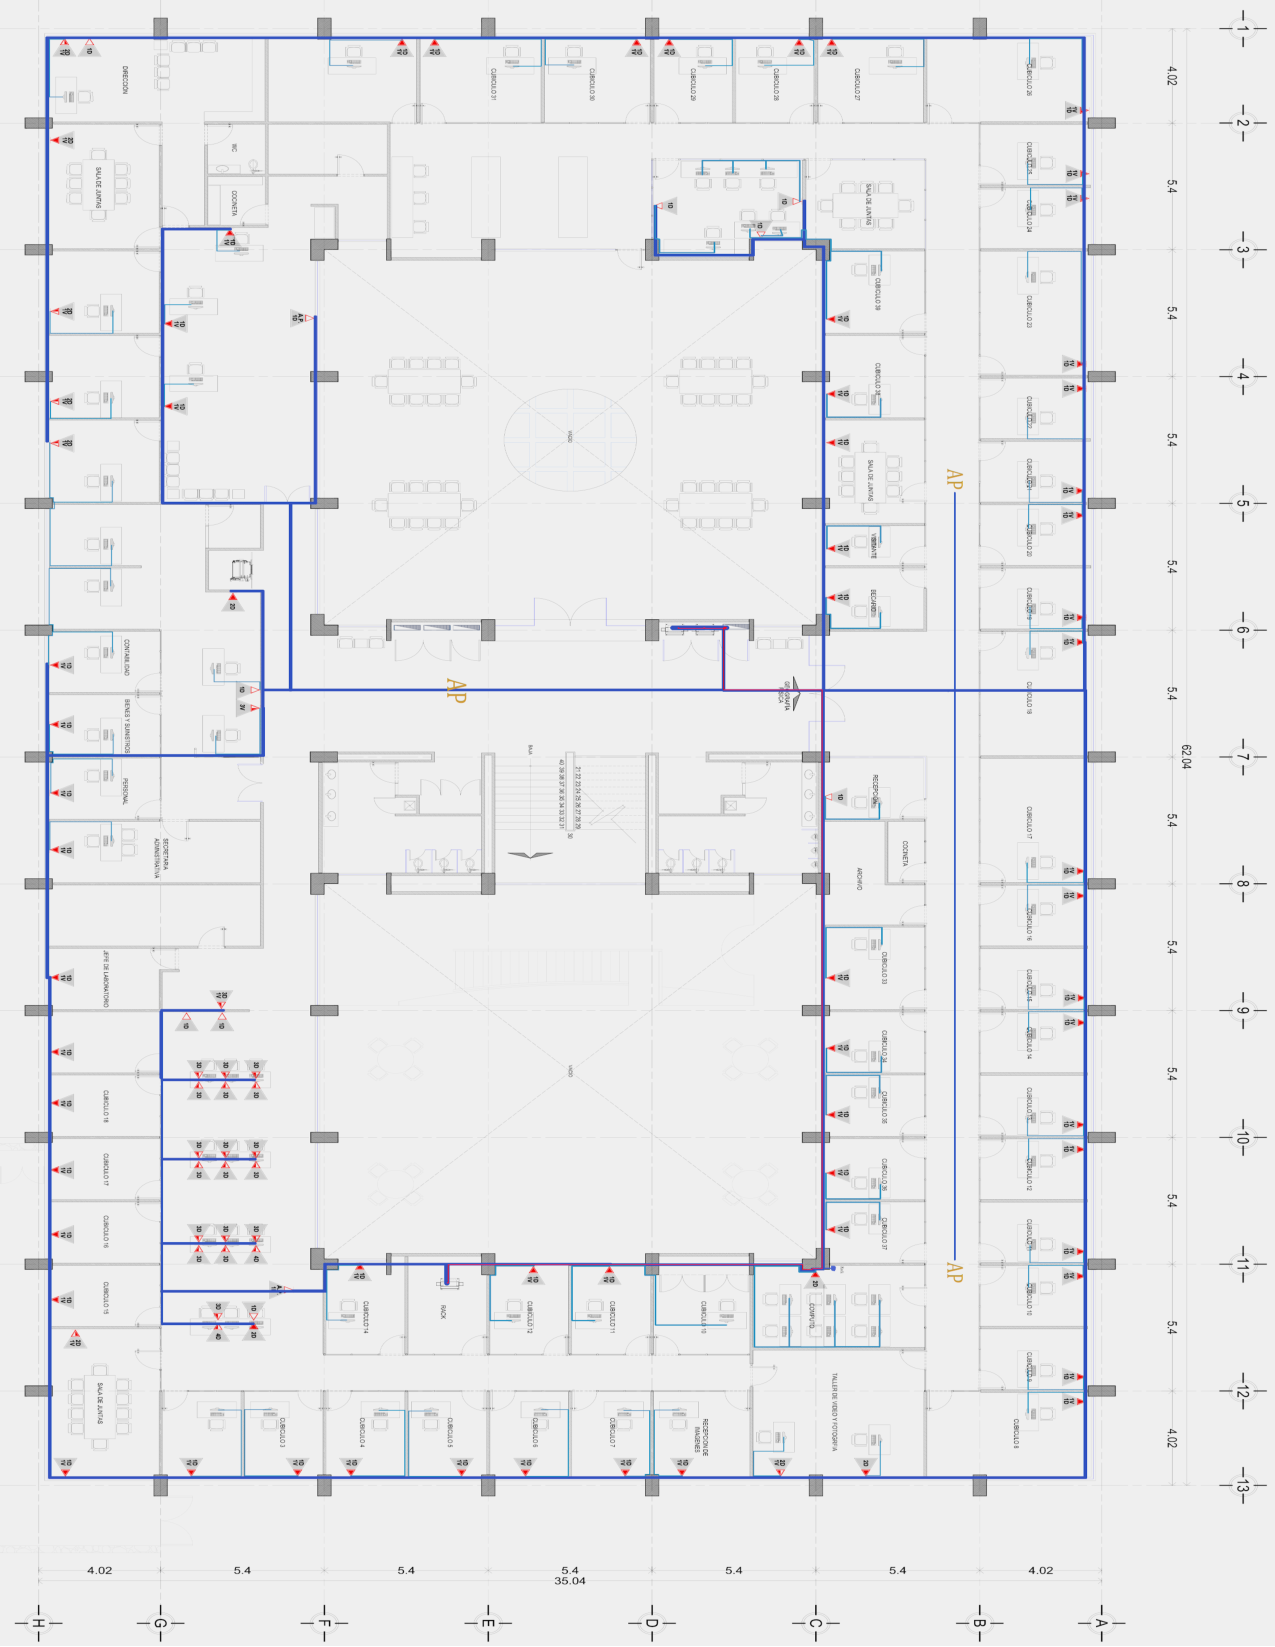
\includepdf{img/2p-mod.pdf}\label{page:plano}

\newpage{}

\printglossary[type=\acronymtype]

\printglossary{}

\newpage{}

\listoftables
%\addcontentsline{toc}{chapter}{\listtablename}
\listoffigures


\end{document}
